\documentclass{standalone}
\usepackage{tikz}
\usetikzlibrary{patterns, positioning}


\begin{document}
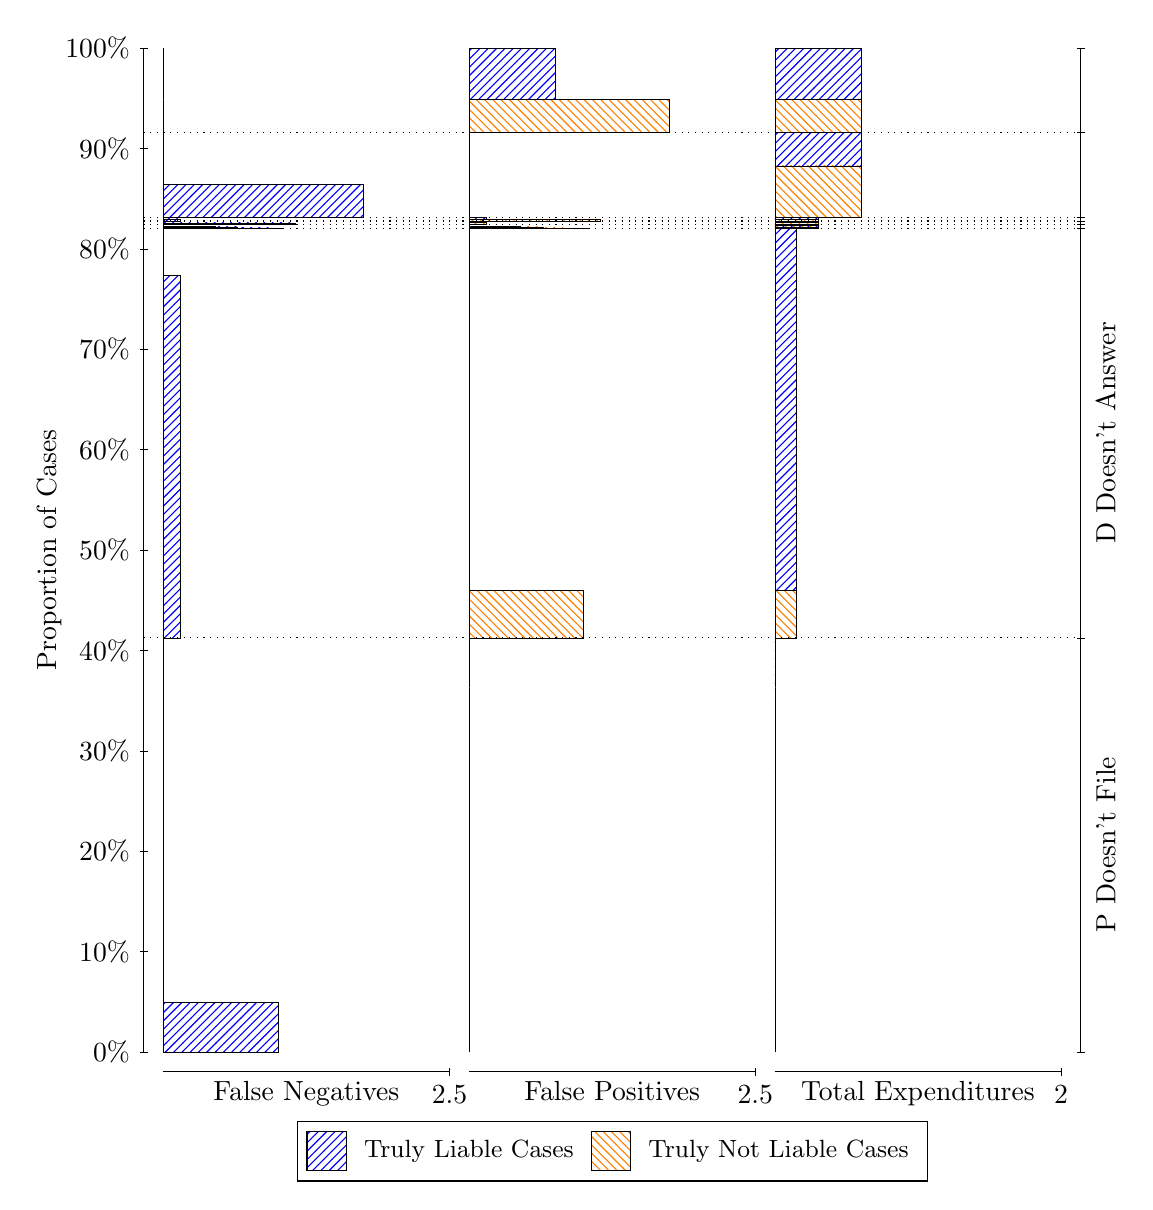
\begin{tikzpicture}
\draw[black, very thin] (1.5,1.75) -- (1.5,14.5);
\node[rotate=90, text=black, anchor=center] at (0.3, 8.125) {Proportion of Cases};
\draw[black, very thin] (1.45,1.75) -- (1.55,1.75);
\node[text=black, anchor=east] at (1.45, 1.75) {0\%};
\draw[black, very thin] (1.45,3.025) -- (1.55,3.025);
\node[text=black, anchor=east] at (1.45, 3.025) {10\%};
\draw[black, very thin] (1.45,4.3) -- (1.55,4.3);
\node[text=black, anchor=east] at (1.45, 4.3) {20\%};
\draw[black, very thin] (1.45,5.575) -- (1.55,5.575);
\node[text=black, anchor=east] at (1.45, 5.575) {30\%};
\draw[black, very thin] (1.45,6.85) -- (1.55,6.85);
\node[text=black, anchor=east] at (1.45, 6.85) {40\%};
\draw[black, very thin] (1.45,8.125) -- (1.55,8.125);
\node[text=black, anchor=east] at (1.45, 8.125) {50\%};
\draw[black, very thin] (1.45,9.4) -- (1.55,9.4);
\node[text=black, anchor=east] at (1.45, 9.4) {60\%};
\draw[black, very thin] (1.45,10.675) -- (1.55,10.675);
\node[text=black, anchor=east] at (1.45, 10.675) {70\%};
\draw[black, very thin] (1.45,11.95) -- (1.55,11.95);
\node[text=black, anchor=east] at (1.45, 11.95) {80\%};
\draw[black, very thin] (1.45,13.225) -- (1.55,13.225);
\node[text=black, anchor=east] at (1.45, 13.225) {90\%};
\draw[black, very thin] (1.45,14.5) -- (1.55,14.5);
\node[text=black, anchor=east] at (1.45, 14.5) {100\%};

\draw[black, very thin] (13.4,1.75) -- (13.4,14.5);
\draw[black, very thin] (13.35,1.75) -- (13.45,1.75);
\node[anchor=west] at (13.35, 1.75) {};
\draw[black, very thin] (13.35,7.01) -- (13.45,7.01);
\node[anchor=west] at (13.35, 7.01) {};
\draw[black, very thin] (13.35,12.211) -- (13.45,12.211);
\node[anchor=west] at (13.35, 12.211) {};
\draw[black, very thin] (13.35,12.26) -- (13.45,12.26);
\node[anchor=west] at (13.35, 12.26) {};
\draw[black, very thin] (13.35,12.303) -- (13.45,12.303);
\node[anchor=west] at (13.35, 12.303) {};
\draw[black, very thin] (13.35,12.347) -- (13.45,12.347);
\node[anchor=west] at (13.35, 12.347) {};
\draw[black, very thin] (13.35,13.424) -- (13.45,13.424);
\node[anchor=west] at (13.35, 13.424) {};
\draw[black, very thin] (13.35,14.5) -- (13.45,14.5);
\node[anchor=west] at (13.35, 14.5) {};

\draw[black, very thin, pattern color=blue, pattern=north east lines] (1.75,1.75) rectangle (3.2033,2.3828);
\draw[black, very thin, pattern color=orange, pattern=north west lines] (1.75,2.3828) rectangle (1.75,7.01);
\draw[black, very thin, pattern color=blue, pattern=north east lines] (1.75,7.01) rectangle (1.968,11.608);
\draw[black, very thin, pattern color=orange, pattern=north west lines] (1.75,11.608) rectangle (1.75,12.211);
\draw[black, very thin, pattern color=blue, pattern=north east lines] (1.75,12.211) rectangle (3.276,12.213);
\draw[black, very thin, pattern color=blue, pattern=north east lines] (1.75,12.213) rectangle (3.1307,12.215);
\draw[black, very thin, pattern color=blue, pattern=north east lines] (1.75,12.215) rectangle (2.9853,12.216);
\draw[black, very thin, pattern color=blue, pattern=north east lines] (1.75,12.216) rectangle (2.84,12.217);
\draw[black, very thin, pattern color=blue, pattern=north east lines] (1.75,12.217) rectangle (2.6947,12.229);
\draw[black, very thin, pattern color=blue, pattern=north east lines] (1.75,12.229) rectangle (2.5493,12.229);
\draw[black, very thin, pattern color=blue, pattern=north east lines] (1.75,12.229) rectangle (2.404,12.231);
\draw[black, very thin, pattern color=blue, pattern=north east lines] (1.75,12.231) rectangle (2.2587,12.232);
\draw[black, very thin, pattern color=blue, pattern=north east lines] (1.75,12.232) rectangle (2.1133,12.235);
\draw[black, very thin, pattern color=orange, pattern=north west lines] (1.75,12.235) rectangle (1.75,12.26);
\draw[black, very thin, pattern color=blue, pattern=north east lines] (1.75,12.26) rectangle (3.4213,12.278);
\draw[black, very thin, pattern color=orange, pattern=north west lines] (1.75,12.278) rectangle (1.75,12.303);
\draw[black, very thin, pattern color=blue, pattern=north east lines] (1.75,12.303) rectangle (1.968,12.329);
\draw[black, very thin, pattern color=orange, pattern=north west lines] (1.75,12.329) rectangle (1.75,12.347);
\draw[black, very thin, pattern color=blue, pattern=north east lines] (1.75,12.347) rectangle (4.2933,12.767);
\draw[black, very thin, pattern color=orange, pattern=north west lines] (1.75,12.767) rectangle (1.75,13.424);
\draw[black, very thin, pattern color=orange, pattern=north west lines] (1.75,13.424) rectangle (1.75,13.844);
\draw[black, very thin, pattern color=blue, pattern=north east lines] (1.75,13.844) rectangle (1.75,14.5);
\draw[black, very thin, pattern color=orange, pattern=north west lines] (5.6333,1.75) rectangle (5.6333,6.3773);
\draw[black, very thin, pattern color=blue, pattern=north east lines] (5.6333,6.3773) rectangle (5.6333,7.01);
\draw[black, very thin, pattern color=orange, pattern=north west lines] (5.6333,7.01) rectangle (7.0867,7.6132);
\draw[black, very thin, pattern color=blue, pattern=north east lines] (5.6333,7.6132) rectangle (5.6333,12.211);
\draw[black, very thin, pattern color=orange, pattern=north west lines] (5.6333,12.211) rectangle (7.1593,12.213);
\draw[black, very thin, pattern color=orange, pattern=north west lines] (5.6333,12.213) rectangle (7.014,12.214);
\draw[black, very thin, pattern color=orange, pattern=north west lines] (5.6333,12.214) rectangle (6.8687,12.216);
\draw[black, very thin, pattern color=orange, pattern=north west lines] (5.6333,12.216) rectangle (6.7233,12.216);
\draw[black, very thin, pattern color=orange, pattern=north west lines] (5.6333,12.216) rectangle (6.578,12.228);
\draw[black, very thin, pattern color=orange, pattern=north west lines] (5.6333,12.228) rectangle (6.4327,12.229);
\draw[black, very thin, pattern color=orange, pattern=north west lines] (5.6333,12.229) rectangle (6.4327,12.229);
\draw[black, very thin, pattern color=orange, pattern=north west lines] (5.6333,12.229) rectangle (6.2873,12.231);
\draw[black, very thin, pattern color=orange, pattern=north west lines] (5.6333,12.231) rectangle (6.142,12.232);
\draw[black, very thin, pattern color=orange, pattern=north west lines] (5.6333,12.232) rectangle (5.9967,12.235);
\draw[black, very thin, pattern color=blue, pattern=north east lines] (5.6333,12.235) rectangle (5.706,12.239);
\draw[black, very thin, pattern color=blue, pattern=north east lines] (5.6333,12.239) rectangle (5.6333,12.26);
\draw[black, very thin, pattern color=orange, pattern=north west lines] (5.6333,12.26) rectangle (5.8513,12.285);
\draw[black, very thin, pattern color=blue, pattern=north east lines] (5.6333,12.285) rectangle (5.6333,12.303);
\draw[black, very thin, pattern color=orange, pattern=north west lines] (5.6333,12.303) rectangle (7.3047,12.322);
\draw[black, very thin, pattern color=blue, pattern=north east lines] (5.6333,12.322) rectangle (5.8513,12.347);
\draw[black, very thin, pattern color=orange, pattern=north west lines] (5.6333,12.347) rectangle (5.6333,13.004);
\draw[black, very thin, pattern color=blue, pattern=north east lines] (5.6333,13.004) rectangle (5.6333,13.424);
\draw[black, very thin, pattern color=orange, pattern=north west lines] (5.6333,13.424) rectangle (8.1767,13.844);
\draw[black, very thin, pattern color=blue, pattern=north east lines] (5.6333,13.844) rectangle (6.7233,14.5);
\draw[black, very thin, pattern color=orange, pattern=north west lines] (9.5167,1.75) rectangle (9.5167,6.3773);
\draw[black, very thin, pattern color=blue, pattern=north east lines] (9.5167,6.3773) rectangle (9.5167,7.01);
\draw[black, very thin, pattern color=orange, pattern=north west lines] (9.5167,7.01) rectangle (9.7892,7.6132);
\draw[black, very thin, pattern color=blue, pattern=north east lines] (9.5167,7.6132) rectangle (9.7892,12.211);
\draw[black, very thin, pattern color=orange, pattern=north west lines] (9.5167,12.211) rectangle (10.062,12.229);
\draw[black, very thin, pattern color=blue, pattern=north east lines] (9.5167,12.229) rectangle (10.062,12.248);
\draw[black, very thin, pattern color=orange, pattern=north west lines] (9.5167,12.248) rectangle (10.062,12.252);
\draw[black, very thin, pattern color=blue, pattern=north east lines] (9.5167,12.252) rectangle (10.062,12.254);
\draw[black, very thin, pattern color=orange, pattern=north west lines] (9.5167,12.254) rectangle (10.062,12.257);
\draw[black, very thin, pattern color=blue, pattern=north east lines] (9.5167,12.257) rectangle (10.062,12.26);
\draw[black, very thin, pattern color=orange, pattern=north west lines] (9.5167,12.26) rectangle (10.062,12.285);
\draw[black, very thin, pattern color=blue, pattern=north east lines] (9.5167,12.285) rectangle (10.062,12.303);
\draw[black, very thin, pattern color=orange, pattern=north west lines] (9.5167,12.303) rectangle (10.062,12.322);
\draw[black, very thin, pattern color=blue, pattern=north east lines] (9.5167,12.322) rectangle (10.062,12.347);
\draw[black, very thin, pattern color=orange, pattern=north west lines] (9.5167,12.347) rectangle (10.607,13.004);
\draw[black, very thin, pattern color=blue, pattern=north east lines] (9.5167,13.004) rectangle (10.607,13.424);
\draw[black, very thin, pattern color=orange, pattern=north west lines] (9.5167,13.424) rectangle (10.607,13.844);
\draw[black, very thin, pattern color=blue, pattern=north east lines] (9.5167,13.844) rectangle (10.607,14.5);
\draw[black, dotted] (1.5,7.01) -- (13.4,7.01);
\draw[black, dotted] (1.5,12.211) -- (13.4,12.211);
\draw[black, dotted] (1.5,12.26) -- (13.4,12.26);
\draw[black, dotted] (1.5,12.303) -- (13.4,12.303);
\draw[black, dotted] (1.5,12.347) -- (13.4,12.347);
\draw[black, dotted] (1.5,13.424) -- (13.4,13.424);
\draw[black, very thin] (1.75,1.5) -- (5.3833,1.5);
\node[text=black, anchor=north] at (3.5667, 1.5) {False Negatives};
\draw[black, very thin] (5.3833,1.45) -- (5.3833,1.55);
\node[text=black, anchor=north] at (5.3833, 1.45) {2.5};

\draw[black, very thin] (5.6333,1.5) -- (9.2667,1.5);
\node[text=black, anchor=north] at (7.45, 1.5) {False Positives};
\draw[black, very thin] (9.2667,1.45) -- (9.2667,1.55);
\node[text=black, anchor=north] at (9.2667, 1.45) {2.5};

\draw[black, very thin] (9.5167,1.5) -- (13.15,1.5);
\node[text=black, anchor=north] at (11.333, 1.5) {Total Expenditures};
\draw[black, very thin] (13.15,1.45) -- (13.15,1.55);
\node[text=black, anchor=north] at (13.15, 1.45) {2};

\node[text=black, centered, rotate=90] at (13.72, 4.38) {P Doesn't File};
\node[text=black, centered, rotate=90] at (13.72, 9.6105) {D Doesn't Answer};






\draw (7.449999999999999,1.5) node[draw=none] (baseCoordinate) {};
\begin{scope}[align=center]
        \matrix[scale=0.5, draw=black, below=0.5cm of baseCoordinate, nodes={draw}, column sep=0.1cm]{
            \node[rectangle, draw, minimum width=0.5cm, minimum height=0.5cm, pattern color=blue, pattern=north east lines] {}; &
            \node[draw=none, font=\small, text=black] (B) {Truly Liable Cases}; &
            \node[rectangle, draw, minimum width=0.5cm, minimum height=0.5cm, pattern color=orange, pattern=north west lines] {}; &
            \node[draw=none, font=\small, text=black] (B) {Truly Not Liable Cases}; \\
            };
\end{scope}

\end{tikzpicture}
\end{document}